% !TeX root = skripta-konstitutivni-vztahy.tex
% !TeX lastmodified = 2018-11-20

\subsection{Entropická elasticita}
Při teplotě absolutní nuly jakékoli vlákno (řetězec, makromolekula) zaujímá tvar minimalizující jeho energii, což odpovídá přímému prutu, pokud rozhodující veličinou je celková deformační energie včetně energie vynaložené na ohybovou deformaci vlákna $W_\text{bend}$
\begin{equation}
	W_\text{bend} = \left(\frac{K_f}{2}\right) \int\limits_0^L \left(\frac{\partial t}{\partial s}\right)^2 \diff s,
\end{equation}
kde
\begin{description}
	\item[$K_f = EJ$] je ohybová tuhost vlákna,
	\item[$\diff s$] element délky vlákna (křivočarý),
	\item[$L$] (contour length) je celková křivočará délka vlákna (rovná vzdálenosti jeho konců v napřímeném tvaru),
	\item[$\tfrac{\partial t}{\partial s}$] je rychlost změny tečného vektoru podél délky~$s$ vlákna (lokální křivost).
\end{description}

\begin{figure}[H]
	\centering
	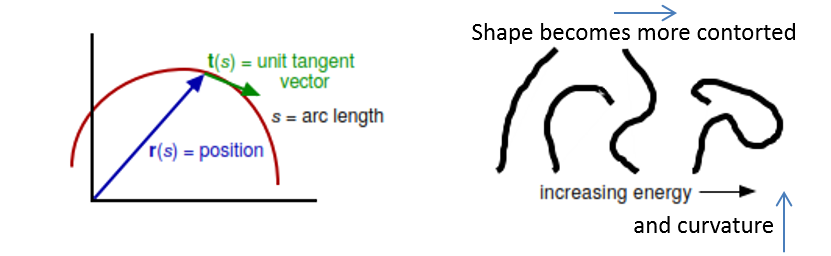
\includegraphics{entropicka-elasticita}
	\caption{Entropická elasticita}
	\label{fig:entropicka-elasticita}
\end{figure}

\subsubsection{Entropie}
Entropie $S$ je mírou pravděpodobnosti daného stavu; v~termodynamice vratných dějů je definována následovně:
\begin{equation}
	\diff S := \frac{\diff Q}{T}
\end{equation}

Pro makromolekulární řetězec je entropie definována pomocí maximálního počtu dosažitelných (tvarových) konfigurací:
\begin{equation}
	S := \ln\left(\text{maximální počet možných konfigurací}\right)
\end{equation}

S~rostoucí entropií určitého tvaru tedy roste pravděpodobnost, že se tento tvar řetězce reálně vyskytne.
Pak pravděpodobnost $P(E)$, že vlákno s~určitou energií $W_\text{bend}$ se vyskytne právě v~určité specifické konfiguraci (tvaru), lze vyjádřit vztahem
\begin{equation}
	P(E) = \exp\left(-\frac{W_\text{bend}}{k_B T}\right),
\end{equation}
kde pravá strana vyjadřuje Boltzmannův faktor\footnote{Fung, YC, 1993}\footnote{Boal, MC, 2002}.

S~rostoucí entropií určitého tvaru roste pravděpodobnost, že se tento tvar řetězce reálně vyskytne.
Pro látky s~nezanedbatelným vlivem entropie na elastické chování není rozhodující veličinou samotná deformační energie, ale Gibbsova volná energie.

\subsubsection{Gibbsova a~Helmholtzova volná energie $G$}
je největší množství energie uchované v soustavě za izotermických a~izobarických (Gibbsova) nebo izovolumických (Helmholtzova) podmínek.

\begin{itemize}
	\item Gibbsova volná energie -- Termodynamika plynů a~par (konstantní tlak)
	\begin{equation}
	\Delta G = \Delta H - T \Delta S,
	\end{equation}
	\item Gibbsova volná energie -- Obecný tvar pro všechna skupenství
	\begin{equation}
	\Delta G = \Delta E + p \Delta V - T \Delta S,
	\end{equation}
	\item Helmholtzova volná energie -- Tvar platný pro tuhé skupenství (konstantní objem)
	\begin{equation}
	\Delta G = \Delta E - T \Delta S,
	\end{equation}
\end{itemize}
kde
\begin{description}
	\item[$H$] je entalpie,
	\item[$E$] je vnitřní  energie,
	\item[$T$] je absolutní teplota,
	\item[$p$] je tlak,
	\item[$V$] je objem (pro látky v tuhém skupenství považován za konstantní)
\end{description}

Pro izotermický děj odpovídá minimalizace volné energie spontánnímu procesu, tj. $\Delta G < 0$ s~nárůstem entropie.
Je-li však vlákno natahováno, klesá počet možných konfigurací (na jedinou v~plně napřímené konfiguraci), tedy klesá i~entropie, což odpovídá procesu nespontánnímu, tj. $\Delta G > 0$.
\footnote{[2] Boal, MC, 2002; [3] Sean, E, 2010; [6] Mofrad , CM, 2006; [15] Mucke, JMB, 2004}

\subsubsection{Perzistentní délka -- délka stálosti tvaru}
Při nenulové absolutní teplotě $T$ dochází k~ohybu přímé tyče vlivem výměny energie s~okolím (u~molekul Brownův pohyb).
Perzistentní délka (persistence length) $L_p$ určuje délku, pod níž se (molekulární) řetězec chová jako tyč s +významnou ohybovou tuhostí, zatímco při délkách větších než $L_p$ se chová jako ohebné vlákno.
\begin{equation}
	L_p = \frac{K_f}{k_B T} = \frac{E J}{k_B T} = \frac{E}{k_B T} \left(\frac{\pi}{64} d^4\right),
\end{equation}
kde
\begin{itemize}
	\item[$E$] je Youngův modul,
	\item[$d$] je průměr vlákna,
	\item[$J$] je kvadratický moment.
\end{itemize}
Pak u~řetězce dochází k teplotním tvarovým fluktuacím; jeho tvar není jednoznačný, ale různé tvary jsou zaujímány s~různou pravděpodobností.

$L \ll L_p$ (tuhá tyč):
\begin{itemize}
	\item Řetězec se jeví přímý a~poměrně tuhý (prut).
	\item Pro jeho chování je rozhodující ohybová energie, bez vlivu entropie.
\end{itemize}

$L \gg L_p$ (ohebné vlákno) nebo $L \sim L_p$ (poloohebné vlákno):
\begin{itemize}
	\item Řetězec zaujímá spíše zakřivené tvary a~jeví se jako ohebné vlákno.
	\item Fluktuace tvaru a~následně energie v~termodynamické rovnováze se stávají významnými a~entropická elasticita se stává rozhodující (elastomery).
\end{itemize}

\subsubsection{Entalpická a~entropická elasticita}
Pro krystalické látky vnější zatížení mění rovnovážné meziatomární vzdálenosti a~zvyšuje vnitřní energii krystalu (entalpická elasticita).

Dlouhé ohebné molekuly elastomeru (gumy) jsou zakřivené a~tepelná energie je udržuje ve stálém termálním pohybu. Následně se s~deformací mění jejich entropie a~vzniká elastické napětí (entropická elasticita).

Z~porovnání entalpie, vnitřní energie a~volné energie plyne, že pokud je příspěvek entropické elasticity zanedbatelný, redukuje se uvedený přístup na entalpickou („klasickou“) elasticitu, obvyklou u~krystalických látek.
Pokud je příspěvek entropické elasticity dominantní (u~elastomerů), pak nárůst entropie (přirozený proces) odpovídá poklesu entalpie, resp. vnitřní energie (přirozený proces).

Entropická elasticita pocházející od protahování jednotlivých vláken termálními fluktuacemi se projevuje silnou nelinearitou.
Proto silné deformační zpevnění struktury je považováno za známku entropické elasticity.

\subsubsection{Entropická elasticita u~jednovláknového polymeru}
Při nulové teplotě $L_p \gg L$
\begin{figure}[H]
	\centering
	
\includegraphics[height=2cm]{jednovlaknovy-polymer-nulova-teplota}
	\caption{Jednovláknový kompozit při nulové teplotě}
	\label{fig:jednovlaknovy-polymer-nulova-teplota}
\end{figure}
Ohybová tuhost
\begin{equation}
	K_f = L_p K_B T
\end{equation}

Při nenulové teplotě $L_p \ll L$
\begin{figure}[H]
	\centering
	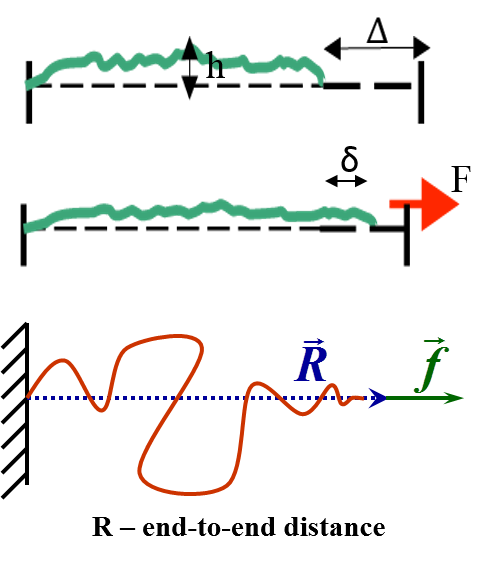
\includegraphics{jednovlaknovy-polymer-nenulova-teplota}
	\caption{Jednovláknový kompozit při nenulové teplotě}
	\label{fig:jednovlaknovy-polymer-nenulova-teplota}
\end{figure}

Síla $f$ se rovná derivaci Gibbsovy volné energie podle $R$
\footnote{[2] Boal, Mechanics of the Cell, 2002; [17] Bustamante, Science, 1994}
\begin{equation}
	f = \frac{\delta G}{\delta R} = \frac{3 K_B T R}{L_p L}
\end{equation}

\subsubsection{Původ elasticity pro různé materiály}
\begin{figure}[H]
	\centering
	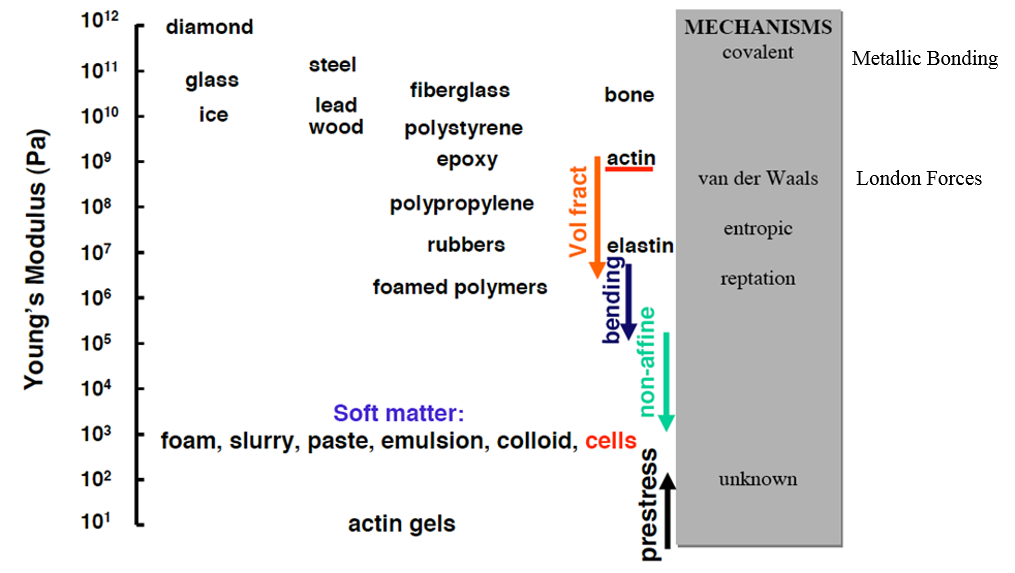
\includegraphics[width=0.7\linewidth]{elasticita-materialu}
	\caption{Elasticita různých materiálů}
	\label{fig:elasticita-materialu}
\end{figure}

Pro krystalické látky vnější zatížení mění rovnovážné meziatomární vzdálenosti a~zvyšuje vnitřní energii krystalu (entalpická elasticita).

Dlouhé ohebné molekuly gumy jsou zakřivené a~tepelná energie je udržuje ve stálém termálním pohybu.
Následně se s deformací mění jejich entropie a~vzniká elastické napětí (entropická elasticita).\footnote{[1] Fung ,B, 1993; [2] Boal , MC, 2002; [6] Mofrad , CM, 2006; [24] Fabry, CGM, 2003}
